 \documentclass[letter,12pt]{article}
%
\usepackage[left=1in, top=1in, bottom=1in, right=1in]{geometry}

% packages 
\usepackage{latexsym,amssymb,amsmath,color}
%\usepackage{theorem}
\usepackage{graphicx}
%\usepackage[colorlinks=true]{hyperref}
%\hypersetup{urlcolor=blue, citecolor=red}
%\usepackage{algorithmic}
%\usepackage{algorithm}
\usepackage{cite}
\usepackage{verbatim}
\usepackage[table]{xcolor}

% -------------- macros
\newcommand{\p}{\partial}
\def\Cb{\overline{C}}

\newcommand{\R}{\mathbb{R}}
\newcommand{\N}{\mathbb{N}}
\newcommand{\cov}{\mathrm{cov}}
\newcommand{\iid}{\stackrel{iid}{\sim}}
\newcommand{\F}{\mathcal{F}}%
\newcommand{\be}{\begin{equation}}
\newcommand{\ee}{\end{equation}}
\newcommand{\bea}{\begin{eqnarray}}
\newcommand{\eea}{\end{eqnarray}}
%\newcommand{\p}{\partial}
\newcommand{\ttt}{\tilde}
%
\def\Wb{\overline{W}}
\def\td{\tilde \delta}
\def\tL{\tilde L}
\def\tU{\tilde U}
\def\tt{\tilde t}
\def\Vector#1{\mbox{\boldmath $#1$}}
\def\vH{{\Vector H}}
\def\vx{{\Vector x}}
\def\vy{{\Vector y}}
\def\vz{{\Vector z}}
\def\vj{{\Vector j}}
\def\vk{{\Vector k}}
\def\vt{{\Vector t}}
\def\ve{{\Vector e}}
\def\vb{{\Vector b}}
\def\vg{{\Vector g}}
\def\vn{{\Vector n}}
\def\vp{{\Vector p}}
\def\vr{{\Vector r}}
\def\vS{{\Vector S}}
\def\vV{{\Vector V}}
\def\vY{{\Vector Y}}
\def\vX{{\Vector X}}
\def\vv{{\Vector v}}
\def\vu{{\Vector u}}
\def\vQ{{\Vector Q}}
\def\vZ{{\Vector Z}}
\def\vN{{\Vector N}}
\def\vF{{\Vector F}}
\def\vC{{\Vector C}}
\def\vq{{\Vector q}}
\def\vom{{\Vector \omega}}
\def\vtau{{\Vector \tau}}
\def\F{{\rm\bf F}}
\def\sech{{\rm sech}}
\def\funnyzeta{\varsigma}
\def\tQ{\stackrel{\ldots}{Q}}
%
\def\Re{{\rm Re}}
\def\Sc{{\rm Sc}}
\def\Pe{{\rm Pe}}
\def\Pr{{\rm Pr}}
\def\Da{{\rm Da}}
\def\rf{{\rm ref}}
\def\eps{{\varepsilon}}
\def\ep{\epsilon'}
\def\O{{\rm O}}
\def\1{{\rm 1}}
\def\so{^{\rm (0)}}
\def\s1{^{\rm (1)}}
\def\d{{\rm d}}
\def\ttm{^{{\rm ttm}}}
\def\img{^{\rm im}}
\def\si{^{\rm si}}
%
\def\ol{\overline}
%
\def\tn{^{n}}
\def\tnm{^{n-1}}
\def\new#1{{\bf #1}}
%\def\new#1{{#1}}

\renewcommand{\L}{\mathcal{L}}
\newcommand{\Q}{\mathcal{Q}}
\newcommand{\U}{\mathcal{U}}
\newcommand{\G}{\mathcal{N}}
\newcommand{\V}{\mathcal{V}}
\renewcommand{\P}{\mathrm{P}}
\newcommand{\B}{\mathcal{B}}
\renewcommand{\vec}[1]{{\mathchoice
                     {\mbox{\boldmath$\displaystyle{#1}$}}
                     {\mbox{\boldmath$\textstyle{#1}$}}
                     {\mbox{\boldmath$\scriptstyle{#1}$}}
                     {\mbox{\boldmath$\scriptscriptstyle{#1}$}}}}
\newcommand{\var}[1]{{\mathrm{Var}}\left( {#1} \right)}
\newcommand{\normim}[1]{\left\| {#1} \right\|_{\scriptscriptstyle L^{2}(\Omega^{*})}}
\newcommand{\avemu}[1]{\mathrm{E}\left({#1}\right)}
\newcommand{\ave}[1]{\left\langle {#1} \right\rangle}
\newcommand{\prob}[1]{\mathrm{Prob}\left\{ {#1} \right\}}
\newcommand{\ind}[1]{\mathrm{\chi}_{\scriptscriptstyle {#1} }}
\newcommand{\NISP}{\mathcal{S}}
\newcommand{\xxi}{\vec{\xi}}
\newcommand{\ip}[2]{\left( {#1}, {#2} \right)}
\newcommand{\ipmu}[2]{\left( {#1}, {#2} \right)_\mu}
\newcommand{\norm}[1]{\left\| {#1} \right\|_{\scriptscriptstyle L^{2}(\Omega)}}
\newcommand{\normone}[1]{\left\| {#1} \right\|_{\scriptscriptstyle 1}}
\newcommand{\pard}[2]{\frac{\partial{#1}}{\partial{#2}}}
%
%\newcommand{\be}{\begin{equation}}
%\newcommand{\ee}{\end{equation}}
%\newcommand{\bea}{\begin{eqnarray}}
%\newcommand{\eea}{\end{eqnarray}}
%\newcommand{\p}{\partial}
%\newcommand{\ttt}{\tilde}
%
\def\Wb{\overline{W}}
\def\td{\tilde \delta}
\def\tL{\tilde L}
\def\tU{\tilde U}
\def\tt{\tilde t}
\def\Vector#1{\mbox{\boldmath $#1$}}
\def\vH{{\Vector H}}
\def\vx{{\Vector x}}
\def\vy{{\Vector y}}
\def\vz{{\Vector z}}
\def\vj{{\Vector j}}
\def\vk{{\Vector k}}
\def\vt{{\Vector t}}
\def\ve{{\Vector e}}
\def\vb{{\Vector b}}
\def\vg{{\Vector g}}
\def\vn{{\Vector n}}
\def\vp{{\Vector p}}
\def\vr{{\Vector r}}
\def\vS{{\Vector S}}
\def\vV{{\Vector V}}
\def\vY{{\Vector Y}}
\def\vX{{\Vector X}}
\def\vv{{\Vector v}}
\def\vu{{\Vector u}}
\def\vQ{{\Vector Q}}
\def\vZ{{\Vector Z}}
\def\vN{{\Vector N}}
\def\vF{{\Vector F}}
\def\vC{{\Vector C}}
\def\vq{{\Vector q}}
\def\vom{{\Vector \omega}}
\def\vtau{{\Vector \tau}}
\def\F{{\rm\bf F}}
\def\sech{{\rm sech}}
\def\funnyzeta{\varsigma}
\def\tQ{\stackrel{\ldots}{Q}}
%
\def\Re{{\rm Re}}
\def\Sc{{\rm Sc}}
\def\Pe{{\rm Pe}}
\def\Pr{{\rm Pr}}
\def\Da{{\rm Da}}
\def\rf{{\rm ref}}
\def\eps{{\varepsilon}}
\def\ep{\epsilon'}
\def\O{{\rm O}}
\def\1{{\rm 1}}
\def\so{^{\rm (0)}}
\def\s1{^{\rm (1)}}
\def\d{{\rm d}}
\def\ttm{^{{\rm ttm}}}
\def\img{^{\rm im}}
\def\si{^{\rm si}}
%
\def\ol{\overline}
%
\def\tn{^{n}}
\def\tnm{^{n-1}}
\def\new#1{{\bf #1}}
\newcommand{\todo}[1]{\scshape\color{red}{#1}}
%
 \def\ol{\overline}
 \def\no{\noindent}
 \def\qd{\dot{Q}}
% ----------------- end macros

\usepackage[table]{xcolor}
\usepackage{relsize}
\usepackage{bm}
\usepackage{mathrsfs}

 \def\ol{\overline}
 \def\no{\noindent}
 \def\qd{\dot{Q}}

%%%%%%%FLOW DIAGRAM%%%%%%%%%%
\usepackage[latin1]{inputenc}
\usepackage{tikz}
%\usepackage[table]{xcolor}
\usetikzlibrary{shapes,arrows}
% Define block styles
\tikzstyle{decision} = [diamond, draw, fill=blue!20, 
   text width=5.0em, text badly centered, node distance=3cm, inner sep=0pt]
\tikzstyle{block} = [rectangle, draw, fill=cyan!20, 
   text width=9.0em, text centered, rounded corners]
\tikzstyle{line} = [draw, -latex']
\tikzstyle{cloud} = [draw, ellipse,fill=red!20, node distance=3cm,
   minimum height=2em]
%%%%%%%%%%%%%%%%%%%%%%%%%%

%-------------------------------------------------------------------
\begin{document}

\begin{center}
\textsc{
Derivative-based global sensitivity approach to efficient surrogate modelling
with Polynomial Chaos
}

\bigskip 
\bigskip 

Manav Vohra$^{1}$, Alen Alexanderian$^{2}$, Cosmin Safta$^{3}$, Sankaran Mahadevan$^{1}$

\bigskip
\bigskip

\normalsize
$^1$Department of Civil and Environmental Engineering\\
Vanderbilt University\\
Nashville, TN 37235\\

\bigskip

$^2$Department of Mathematics\\
North Carolina State University\\
Raleigh, NC 27695\\

\bigskip

$^3$Sandia National Laboratories\\
Livermore, CA 94550\\

\end{center}

\vspace{6cm}

\begin{tabbing}
Corresponding Author: \hspace{5mm} \= Sankaran Mahadevan\\
       \>  Department of Civil and Environmental Engineering\\
       \>  Vanderbilt University\\
       \>  272 Jacobs Hall, VU Mailbox: PMB 351831 \\
       \>  Nashville, TN 37235 \\
       \> \\
Phone: \> (615) 322-3040 \\
Fax:   \> (615) 343-3773 \\
Email: \>  sankaran.mahadevan@vanderbilt.edu   \\
\\
Submitted to: \> \textit{Reliability Engineering and System Safety} \\
\>  May 2018\\

\bigskip
\end{tabbing}

\clearpage



\tableofcontents

\section{Introduction}
\label{sec:intro}

%\begin{enumerate}
%\item Need for efficient Surrogates - especially for complex models to enable forward UQ, 
%sensitivity studies, calibration, and experimental design (Include citations).
%\item Computational Hurdles: Polynomial Chaos and GP can be computationally 
%intractable and suffer from the curse of dimensionality (Include plots for PCE
%to motivate dimension reduction with citations for both PCE and GP).
%\item Sensitivity analyis - a potent tool for dimension reduction. However, SA can be
%computationally prohibitive. In fact, there are studies demonstrating the use of 
%surrogates to reduce costs associated with SA (include citations). 
%\item DGSM - brief introduction and citations. 
%\item Key contributions of the paper: 1) Methodology that exploits DGSM to reduce the
%dimensionality of the problem and thus enables efficient construction of surrogates.
%2) Application of the proposed methodology to investigate relative importance of
%parameters in the stillinger-weber potential, commonly used for studying phonon transport in silicon. Further, construct a reasonably accurate PC surrogate in the reduced 
%space and demonstrate computational advantage of this approach. .
%\end{enumerate}

The emerging field of uncertainty quantification (UQ) aims at methodologies for 
incorporating, characterizing, quantifying, propagating, and reducing the 
uncertainties associated with predictive models and simulations. For situations
involving complex physical models and compute-intensive simulations, an
efficient approach to construction of model surrogates is sought to enable UQ
in a tractable manner. Polynomial chaos expansion 
(PCE)~\cite{Xiu:2002,Ghanem:2003,Eldred:2008,Olivier:2010} and 
Gaussian Process (GP)~\cite{Rasmussen:2004} or Kriging~\cite{Stein:2012} are
among the most commonly used surrogates for scientific applications. However,
both approaches quickly become prohibitive when the set of uncertain model
inputs and parameters is large-dimensional. Specifically, in the case of a PCE,
a $d$-dimensional polynomial basis with a total order of truncation, $p$ 
requires model realizations at $(p+1)^d$ quadrature nodes to estimate the PC
coefficients using a fully-tensorized Gauss quadrature. This trend is 
illustrated below in Figure~\ref{fig:curse}.

\begin{figure}[htbp]
 \begin{center}
  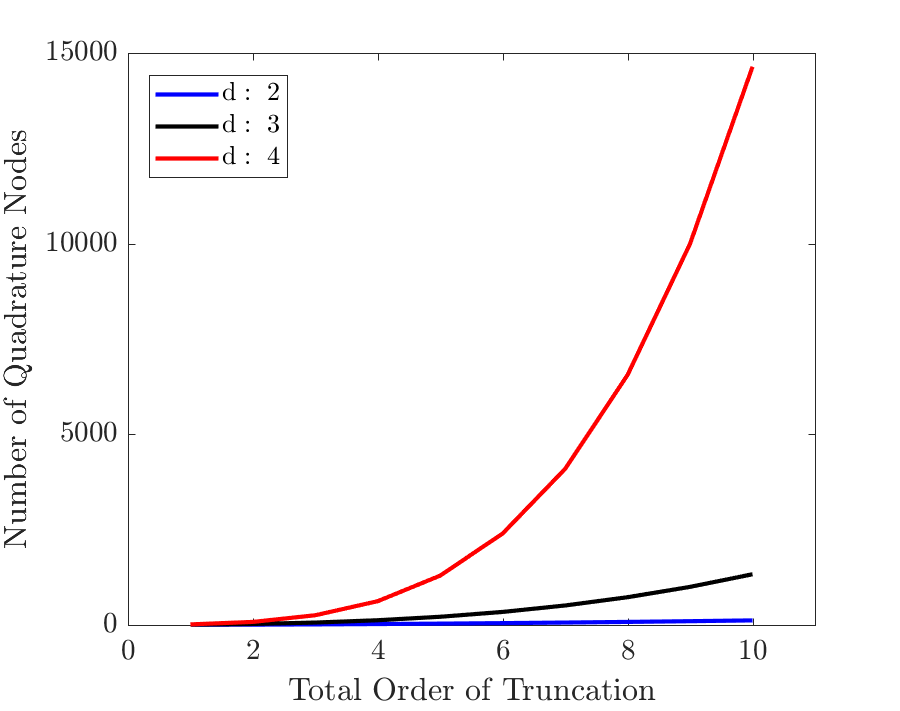
\includegraphics[width=0.70\textwidth]{./Figures/quad_comp}
\caption{Number of fully-tensorized Gauss quadrature nodes ($(p+1)^d$) is plotted against PCE total order truncation, $p$ for $d$ = 2,3, and 4.}
\label{fig:curse}
\end{center}
\end{figure}






\section{Background}
\subsection{DGSM}
\[ 
    \mu_i = E\left(\left( \frac{\partial \mathcal{G}}{\partial \theta_i}\right)^2\right)
          \approx \hat\mu_i := \frac1N\sum_{j = 1}^N 
                  \left(\frac{\partial \mathcal{G}(x_j)}{\partial \theta_i}\right)^2
\]
Can consider variance of $\hat\mu_i$.

\subsection{Polynomial chaos}
\section{Method}

\section{Motivating examples}
\subsection{Borehole: Screening, Convergence, Verification}
\subsection{Semilinear elliptic PDE: Screening, Convergence, Verification}
\subsection{Nonlinear Oscillator: Screening, Convergence, Verification}

\section{Application: Phonon Transport in a Si bar}

Seven uncertain parameters; well-established nominal values exist;
\[
   \theta_i \sim U(\bar\theta_i - \epsilon_i, \bar\theta_i + \epsilon_i), 
   \quad \epsilon_i = 0.1 \bar\theta_i. 
\]
\begin{enumerate}
\item Include all details pertaining to the MD simulation: system, simulation, 
ensembles, etc. 
\item Results
\end{enumerate}

\section{Discussion}
\begin{enumerate}
\item Methodology is agnostic to the choice of surrogate.
\item As required for a PCE, the uncertain parameters need not be independent. 
\item Strategy depends on the application - methodology could be implemented 
sequentially or adaptively. 
\end{enumerate}


\end{document}
